\chapter{Neutron Transport Equation}
\label{chap:neut_transport} % Always give a unique label
% use \chaptermark{}
% to alter or adjust the chapter heading in the running head

\abstract
{
In this chapter, we introduce the \textit{transport equation}, a linearized 
form of the Boltzmann equation suitable for describing neutral particles 
in nuclear systems.  Our goal is to define several fundamental quantities 
needed to describe neutron populations in a reactor in terms of all phase 
space variables. In the next 
chapter, we will derive rather formally the \textit{diffusion equation},
which is the foundation for much of the analysis remaining in this course.  
}

\section{A Look Back}

At this point, we assume the reader has a solid understanding of several 
fundamentals, as covered in Chapters 1-4 in Lewis.  This includes a basic 
familiarity with the various nuclear reactions of interest, such as 
scattering, fission and other resonance reactions, and decay modes, 
along with various neutron sources.  Furthermore, the reader should 
understand microscopic and macroscopic cross-sections, their energy 
dependence, and where each is used.  The basics of energy spectrum 
calculations should be familiar, as should be the path to multigroup 
cross-sections via condensation.  Finally, the reader should have a basic 
appreciation for the various nuclear systems of interest and gross system 
features that fundamentally affect our treatment of the physics.

Our general goal now is to learn how to bring together these concepts to 
model nuclear reactors, and describing the population of neutrons in a 
reactor is our first step toward reaching this goal.

\section{Transport Theory}

Transport theory aims to describe mathematically the movement 
(\textit{i.e} ``tra\-n\-s\-port'') of particles as they traverse a 
medium.  For example, we might describe the transport of high energy 
gammas through a lead shield, or the movement of neutrons through uranium 
dioxide pellets.  We might also describe the movement of particles in a 
dense gas as they navigate through a medium consisting of the gas itself.

In all cases, transport theory describes such processes in an \textit{average} 
sense.  For instance, we do not compute the individual trajectories of 
neutrons in a reactor via transport theory.  That, instead, would require 
molecular dynamics, in which Newton's equation of force is solved for the
many-bodied problem of all neutrons in the vicinity of interest (an 
essentially impossible problem), or perhaps Monte Carlo methods, where a 
sample of individual particles are tracked to approximate ensemble averages 
(a difficult, but tractable problem).  Hence, the quantities we shall 
compute using the equations of transport theory or approximations thereof 
should be recognized as expected and not exact values.

\section{Fundamental Quantities}

We begin by defining several fundamental quantities, all of which apply to 
any neutral particle field. The most fundamental quantity of interest is 
the \textit{phase space density}, knowledge of which we can use to define 
essentially all other relevant quantities:
\begin{center}
  \begin{tabular}{cp{7.0cm}}
    $\bar{n}'''(\vec{r},\vec{v},t)d^3r d^3v \equiv $ &
      expected number of particles in  $d^3r$  about  $\vec{r}$  
      with velocity  $dv$ about  $\vec{v}$ at time $t$.  
  \end{tabular}
\end{center}
Note, in almost any other text, the density is written simply as $n$, 
without bars or primes.  We keep them for consistency  with Lewis.

It is common to break the velocity into its scalar (speed) and vector 
(direction) components.  The scalar component is recast in the energy 
variable via $E = mv^2/2$, and the direction vector is defined 
$\hat{\Omega}=\vec{v}/|\vec{v}|$.  The phase space density can then be 
rewritten as
\begin{center}
  \begin{tabular}{cp{7.0cm}}
    $\bar{n}'''(\vec{r},\hat{\Omega},E,t)d^3r d\Omega dE \equiv $ &
      expected number of particles in  $d^3r$  about  $\vec{r}$  going 
      in the directions $d\Omega$ about $\hat{\Omega}$ with energy  
      $dE$ about  $E$ at time $t$.  
  \end{tabular}
\end{center}
In this form, $\bar{n}'''(\vec{r},\hat{\Omega},E,t)$ is often referred to 
as the \textit{angular density}.  We shall work exclusively with the angular 
density, since many expressions are most conveniently cast in terms of the 
energy $E$.

\begin{figure}[ht]
    \centering
    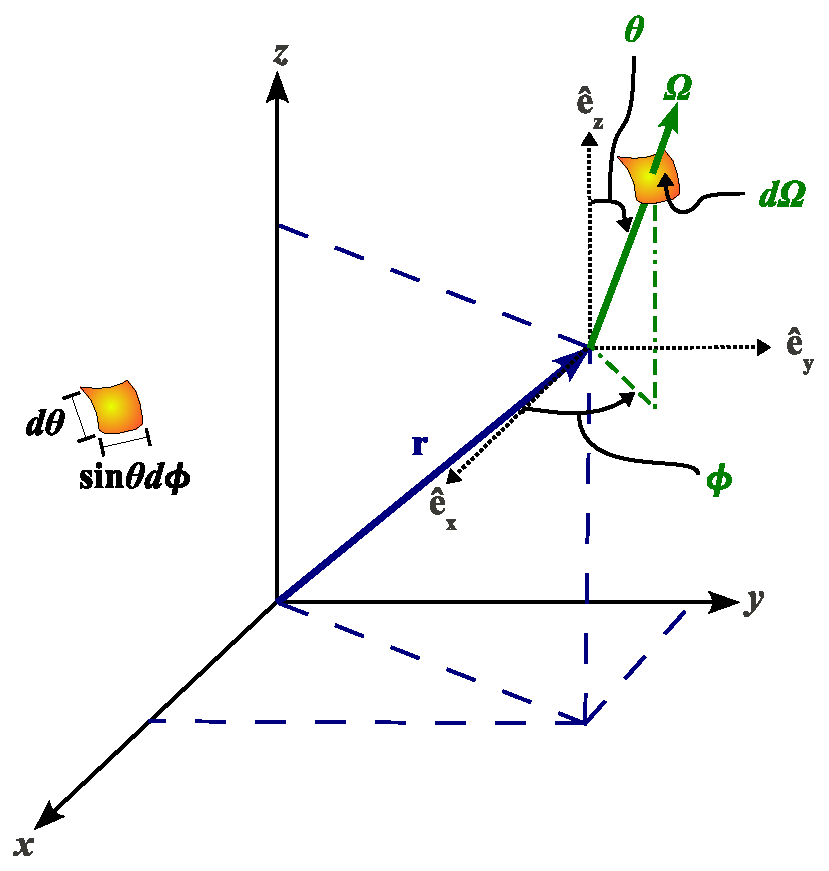
\includegraphics[keepaspectratio, width = 2.7 in]{figs/chap_transport/phase_space}
    \caption{Schematic of Phase Space.}
    \label{fig:phase_space}
\end{figure}

Figure \ref{fig:phase_space} depicts a schematic of the phase space used in 
terms of the position $\vec{r}$ and direction $\hat{\Omega}$.  The position 
vector is further broken down into the polar angle $\theta$ and azimuthal 
angle $\phi$.  The differential solid angle element $d\Omega$ is also shown, 
and can be expressed in terms of $\theta$ and $\phi$ via
\begin{equation*}
 d\Omega = \sin{\theta} d\theta d\phi \, .
\end{equation*}  

In reactor physics, we are frequently interested in volumetric reaction rates 
(for computing power densities, radiation damage, and so forth).  Eq. (3.10) of 
Lewis defines the flux spectrum as
\begin{equation*}
 \varphi(E) = v(E)\bar{n}'''(E) \, ,
\end{equation*}
where $v(E)$ is the speed at energy $E$.  Generalizing to all of phase space, 
we define the \textit{angular flux}
\begin{equation}
   \psi (\vec{r},\hat{\Omega},E,t) = v(E) \bar{n}'''(\vec{r},\hat{\Omega},E,t) \, ,
\label{eq:angularflux}
\end{equation}
and \textit{scalar flux}
\begin{equation}
    \varphi (\vec{r},E,t) = \int_{4\pi} d\Omega \psi (\vec{r},\hat{\Omega},E,t) \, .
\label{eq:scalarflux}
\end{equation}

A quantity closely related to the angular flux is the \textit{angular 
current density},
\begin{equation}
  \vec{j}(\vec{r},\hat{\Omega},E,t) = \hat{\Omega}\psi (\vec{r},\hat{\Omega},E,t)  \, .
\end{equation}
Consider a surface $S$ with outward normal $\hat{e}_S$, and 
let $\vec{S} = \hat{e}_S S$.  Then we have
\begin{center}
  \begin{tabular}{cp{5.0cm}}
    $\vec{j}(\vec{r},\hat{\Omega},E,t) \cdot \vec{S} d\Omega dE \equiv$&
    expected number of particles that cross an area $S$ per second going in the 
    directions $d\Omega$ about $\hat{\Omega}$ with energy  
    $dE$ about  $E$ at time $t$.
  \end{tabular}
\end{center}
A \textit{partial current density} can also be defined with respect to $\vec{S}$:
\begin{center}
  \begin{tabular}{cp{4.3cm}}
    $J_{\pm}(\vec{r},E,t)SdE = 
      \pm \int_{\hat{\Omega} \cdot \hat{e}_S \gtrless 0} d\Omega dE  \vec{S} 
        \cdot \vec{j} (\vec{r},\hat{\Omega},E,t) \equiv $ &
          the rate at which particles in $dE$ about $E$ flow through $S$ in 
          the outward (+) or inward (-) direction at time $t$.
  \end{tabular}
\end{center}

Similarly, the \textit{current density} or just \textit{current} is defined by
 integrating the angular current density over all directions, or
\begin{equation}
 \vec{J}(\vec{r},E,t) = \int_{4\pi} d\Omega \vec{j}(\vec{r},\hat{\Omega},E,t) \, .
\end{equation}
One way to think of the current is as the average direction of flow (the 
vector part) and the net number that flow (magnitude) in that direction 
at a particular point in 
phase space.  More explicitly, we have
\begin{center}
  \begin{tabular}{cp{5.0cm}}
    $\vec{J}(\vec{r},E,t) \cdot \vec{S} dE $ = &
    net number of particles passing outward through $S$ per second with energy 
$dE$ about $E$ at time $t$
  \end{tabular}
\end{center}
From our definition of partial currents, the net current passing outward must 
also be $J_+ - J_-$, yielding the useful identity
\begin{equation}
 \vec{J}(\vec{r},E,t) \cdot \hat{e}_s = J_{+}(\vec{r},E,t) - J_{-}(\vec{r},E,t) \, .
 \label{eq:net2partial}
\end{equation}

%A point of caution: it should be noted that $n$ and $\vec{j}$ must have the same units but represent wholly different things since $n$ is a scalar quantity while $\vec{j}$ is a vector quantity.  This will be true also of $\vec{J}$ and the scalar flux $\phi$, which will be introduced

\section{A General Transport Equation}

Consider an arbitrary volume $V$ with a surface $S$.  Our goal is to represent 
the time rate of change of the neutron 
density $\bar{n}'''(\vec{r},\hat{\Omega},E,t)$ within the volume.  Neglecting
external forces, the only factors affecting the density are collisions within 
the volume that change a particle's velocity, the streaming of particles 
through $S$ into and out of the $V$, and any internal source of particles.  
This simple balance can be expressed mathematically as
\begin{equation}
\begin{split}
 \overbrace{ \frac{\partial}{\partial t} \Bigg ( \int_V d^3r\, \bar{n}'''(\vec{r},\hat{\Omega},E,t) \Bigg ) }^{\text{total rate of change of }\bar{n}'''\text{ in } V} 
      &=  - \overbrace{\int_S dS \hat{e}_S \cdot \vec{j}(\vec{r},\hat{\Omega},E,t) }^{\text{streaming rate}}
       + \overbrace{ \int_V d^3 r \Big( \frac{\partial \bar{n}'''}{\partial t} \Big )_{\mathrm{coll}} }^{\text{collision rate}} \\
      &+ \underbrace{ \int_V d^3 r \, S(\vec{r},\hat{\Omega},E,t) }_{\text{source emission rate}}  \, ,
\end{split}
\label{eq:balance}
\end{equation}
where $S$ represents all sources inside the volume and 
$(\partial \bar{n}'''/\partial t)_{\mathrm{coll}}$ is the time rate 
of change due to collisions, the specific form of which will be discussed 
below.  Note the minus sign on the surface integral, often called the streaming 
term.  Since the integral describes the net rate of neutrons going \textit{out} 
of the surface, we negate it so that a positive net rate directed inward is a 
positive contribution to the total time rate of change of $\bar{n}'''$ in $V$.

Eq. \ref{eq:balance} gives us a simple relation in terms of both volume and 
surface integrals.  Our life is always easiest if we have the same integration 
on both sides.  By the divergence (or Gauss') theorem, we can rewrite the 
streaming term
\begin{equation}
 \int_S dS \hat{e}_S \cdot \vec{j}(\vec{r},\hat{\Omega},E,t) = \int_V d^3r \nabla \cdot \vec{j}(\vec{r},\hat{\Omega},E,t) \, .
\end{equation}
Since $\nabla$ acts on $\vec{r}$ and not $\hat{\Omega}$, we
note $ \nabla \cdot \vec{j} = \nabla \cdot (\hat{\Omega} \bar{n}''') =  
\hat{\Omega} \cdot \nabla \bar{n}''' + \overbrace{ \bar{n}''' \nabla 
\cdot \hat{\Omega}}^{\to 0} = \hat{\Omega} \cdot \nabla \bar{n}'''$.  
Hence, the streaming term becomes
\begin{equation}
 \int_V d^3r \nabla \cdot \vec{j}(\vec{r},\hat{\Omega},E,t) = 
   \int_V d^3r \, \hat{\Omega} \cdot \nabla \bar{n}'''(\vec{r},\hat{\Omega},E,t) \, .
\end{equation}

For a constant volume, $(\partial/\partial t) \int_V d^3 r \, \bar{n}''' = 
\int_V d^3 (\partial \bar{n}'''/\partial t)$, and so our balance equation can 
be rewritten as
\begin{equation}
\begin{split}
 \overbrace{  \Bigg ( \int_V d^3 r \frac{\partial}{\partial t}\bar{n}'''(\vec{r},\hat{\Omega},E,t) \Bigg ) }^{\text{total rate of change of }n\text{ in } V} 
      &=  - \overbrace{\int_V d^3r \hat{\Omega} \cdot \nabla \bar{n}'''(\vec{r},\hat{\Omega},E,t)}^{\text{streaming rate}}
       + \overbrace{ \int_V d^3 r \Big( \frac{\partial \bar{n}'''}{\partial t} \Big )_{\mathrm{coll}} }^{\text{collision rate}} \\
      &+ \underbrace{ \int_V d^3 r \, S(\vec{r},\hat{\Omega},E,t) }_{\text{source emission rate}}  \, .
\end{split}
\label{eq:balance2}
\end{equation}
For an arbitrary volume $V$, the integrands of Eq \ref{eq:balance2} must 
vanish, yielding a general transport equation:
\begin{equation}
  \frac{\partial}{\partial t}\bar{n}'''(\vec{r},\hat{\Omega},E,t) = 
    -\hat{\Omega} \cdot \nabla \bar{n}'''(\vec{r},\hat{\Omega},E,t) + 
    \Big( \frac{\partial n}{\partial t} \Big )_{\mathrm{coll}} +  S(\vec{r},\hat{\Omega},E,t) \, .
\label{eq:general_te}
\end{equation}


\section{Neutron Transport}

The total volumetric collision rate at a particular point in phase space 
and time is simply
\begin{equation}
 R_{\text{coll}}(\vec{r},\hat{\Omega},E,t) = \psi(\vec{r},\hat{\Omega},E,t) \Sigma_t(\vec{r},E) \, .
\end{equation}
Then $R_{\text{coll}}(\vec{r},\hat{\Omega},E,t)d^3r d\Omega dE$ is the rate at 
which neutrons beginning in the differential phase space 
volume $d^3r d\Omega dE$ centered about $(\vec{r},\hat{\Omega},E,t)$ are 
sent to \textit{any} other 
region of phase space by \textit{any} possible mechanism.  The time rate of 
change due to collisions is thus
\begin{equation}
 \Big( \frac{\partial n}{\partial t} \Big )_{\mathrm{coll}} 
   = -\psi(\vec{r},\hat{\Omega},E,t) \Sigma_t(\vec{r},E) \, .
\end{equation}

The source term, $S$, is in general a combination of several contributions, 
including in-scatter, fission, and external sources.  We treat these individually.

When a neutron at one energy and angle scatters, it must end up at a different 
energy and different angle (or else it hasn't scattered).  Then the source 
contribution in one part of phase space due to scattering events in another 
is defined formally as
\begin{equation}
 S_s(\vec{r},\hat{\Omega},E,t) = 
   \int^{\infty}_{0} dE' \int_{4\pi} d\Omega' 
     \Sigma_s(\vec{r},\hat{\Omega}\cdot\hat{\Omega}',E'\to E)
     \psi(\vec{r},\hat{\Omega}',E',t) \, .
\label{eq:q_scatter}
\end{equation}

The volumetric rate of fission neutron production in a system is defined as 
\begin{equation}
 s'''_f(\vec{r},t) = \int^{\infty}_{0} dE' \nu(E')\Sigma_f(\vec{r},E')\varphi(\vec{r},E',t) \, ,
\end{equation}
Recall that fission neutrons appear at a variety of energies, the probability of which 
is denoted $\chi(E)$.  Further recall that fission neutrons are essentially emitted 
isotropically; that is, the outgoing neutrons exhibit no ``memory'' of the incident 
neutron.  Therefore, the fission source can be written
\begin{equation}
 S_f(\vec{r},\hat{\Omega},E,t) = 
   \frac{\chi(E)}{4\pi} \int^{\infty}_{0} dE' \nu(E')\Sigma_f(\vec{r},E')\varphi(\vec{r},E',t) \, .
\label{eq:q_fission}
\end{equation}

However, Eq. \ref{eq:q_fission} is only partially accurate.  Neutrons born 
from fission come in two distinct flavors: those emitted \textit{promptly}, 
and those emitted after some \textit{delay}.  One distinguishes between the 
two through use of the average number of prompt neutrons emitted per 
fission, $\nu_p(E)$ and a prompt fission neutron energy spectrum, $\chi_p(E)$.  
We'll use a special treatment for delayed neutrons in a later chapter.  Worth 
noting is that $\nu$ for delayed neutrons is less than $\nu_p/100$ and that 
the associated $\chi$-spectrum is softer but more erratic. 

For now, we define a \textit{prompt fission source}
\begin{equation}
 S_{fp}(\vec{r},\hat{\Omega},E,t) = 
   \frac{\chi_p(E)}{4\pi} \int^{\infty}_{0} dE' 
   \nu_p(E')\Sigma_f(\vec{r},E')\varphi(\vec{r},E',t) \, ,
\label{eq:q_prompt_fission}
\end{equation}
and denote the \textit{delayed fission source} by 
$S_{fd}(\vec{r},\hat{\Omega},E,t)$ where applicable.

Finally, one can include external sources, represented 
as $S_{e}(\vec{r},\hat{\Omega},E,t)$, and substituting this along with 
Eqs. \ref{eq:q_scatter}, \ref{eq:q_prompt_fission}, and the delayed 
fission source into Eq. \ref{eq:general_te}, we arrive at the 
canonical \textit{neutron transport equation}:
\begin{equation}
  \begin{split}
     \frac{1}{v}\frac{\partial \psi}{\partial t} &+ \hat{\Omega} \cdot \nabla \psi + \Sigma_t(\vec{r},E) \psi(\vec{r},\hat{\Omega},E,t) = \\
           &+ \int^{\infty}_{0} dE' \int_{4\pi} d\Omega' \Sigma_s(\vec{r},\hat{\Omega}\cdot\hat{\Omega}',E'\to E)\psi(\vec{r},\hat{\Omega'},E',t) \\
           &+ \frac{\chi_p(E)}{4\pi} \int^{\infty}_{0} dE' \nu_p(E')\Sigma_f(\vec{r},E')\varphi(\vec{r},E',t) \\
           &+ S_{fd}(\vec{r},\hat{\Omega},E,t)  + S_{e}(\vec{r},\hat{\Omega},E,t) \, .
  \end{split}
  \label{eq:neutron_te}
\end{equation}

\section{Assumptions for the Neutron Transport Equation}
In writing down Eq. \ref{eq:neutron_te} as we have, a number of assumptions 
have been made explicitly or implicitly.  These include:
\begin{enumerate}
   \item The neutron density is large so that it makes sense to be computing 
         for mean values (which is all transport equations can provide).
   \item The neutrons are point particles, meaning that wave effects are insignificant.
   \item Collisions are well-defined, two-body interactions that occur 
         instantaneously. Delayed neutrons from fission, which will be covered 
         in a later chapter, are a notable exception and deserve special treatment.
   \item Between collisions, neutrons stream with a constant velocity.
   \item Neutron-neutron interactions are negligible, which implies that while the 
         population is large enough to make averages meaningful, it's not so large 
         that neutron-neutron collisions become relevant. 
   \item The properties of the medium are assumed known and time-independent. 
         Burnup in a nuclear reactor is an exception, and requires special treatment.
   \item The medium is taken to be isotropic, meaning the cross-sections do not 
         depend on the neutron direction of flight.  Exceptions include crystalline 
         materials, for which the cross-sections can change considerably depending 
         on the direction of flight.  For example, this is true for the graphite 
         structures found in very high temperature reactor (VHTR) designs, 
         and proper treatment of the angular dependence is important.  
\end{enumerate}


\section{Further Reading}
See Duderstadt and Martin \cite{duderstadt1976tt},  Bell and 
Glasstone \cite{bell1970nrt}, and Duderstadt and 
Hamilton \cite{duderstadt1976nra}.